\documentclass[border=4pt]{standalone}
\usepackage{fontspec}
\usepackage{amsmath}
\usepackage{unicode-math}
\setmainfont{Latin Modern Roman}
\setmathfont{Latin Modern Math}
\usepackage{pgfplots}
\usepackage{pgfplotstable}
\pgfplotsset{compat=1.18}
\usepackage{tkz-euclide}
\usetikzlibrary{arrows.meta,calc,angles,quotes,patterns,3d,backgrounds}
\definecolor{ink}{HTML}{123428}
\definecolor{asy}{HTML}{475569}
\definecolor{mint}{HTML}{86e0bd}
\tikzset{asym/.style={asy, line width=0.9pt, dash pattern=on 5pt off 3.5pt},
         guide/.style={gray!70, line width=0.6pt, densely dotted},
         dot/.style={circle, inner sep=0pt, minimum size=5pt, draw=white, line width=0.5pt},
         odot/.style={circle, inner sep=0pt, minimum size=5.5pt, fill=white, line width=1pt},
         lab/.style={font=\footnotesize, inner sep=1.5pt, text=ink}}
\begin{document}
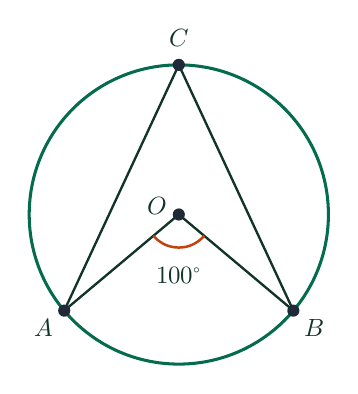
\begin{tikzpicture}
\draw[color={rgb,255:red,4;green,107;blue,77}, line width=1.1pt] (0,0) circle (1.900);
\draw[ink, line width=0.85pt] (0.000,1.900) -- (-1.455,-1.221);
\draw[ink, line width=0.85pt] (0.000,1.900) -- (1.455,-1.221);
\draw[ink, line width=0.85pt] (0.000,0.000) -- (-1.455,-1.221);
\draw[ink, line width=0.85pt] (0.000,0.000) -- (1.455,-1.221);
\draw[color={rgb,255:red,194;green,65;blue,12}, line width=0.9pt] (-0.322,-0.270) -- (-0.297,-0.297) -- (-0.270,-0.322) -- (-0.241,-0.344) -- (-0.210,-0.364) -- (-0.177,-0.381) -- (-0.144,-0.395) -- (-0.109,-0.406) -- (-0.073,-0.414) -- (-0.037,-0.418) -- (-0.000,-0.420) -- (0.037,-0.418) -- (0.073,-0.414) -- (0.109,-0.406) -- (0.144,-0.395) -- (0.177,-0.381) -- (0.210,-0.364) -- (0.241,-0.344) -- (0.270,-0.322) -- (0.297,-0.297) -- (0.322,-0.270);
\node[font=\small, text=ink, inner sep=0.5pt, fill=white] at (-0.000,-0.780) {$100^\circ$};
\fill[color={rgb,255:red,31;green,41;blue,55}] (-1.455,-1.221) circle (2.2pt);
\fill[color={rgb,255:red,31;green,41;blue,55}] (1.455,-1.221) circle (2.2pt);
\fill[color={rgb,255:red,31;green,41;blue,55}] (0.000,1.900) circle (2.2pt);
\fill[color={rgb,255:red,31;green,41;blue,55}] (0.000,0.000) circle (2.2pt);
\node[font=\small, text=ink, inner sep=0.5pt] at (-1.716,-1.440) {$A$};
\node[font=\small, text=ink, inner sep=0.5pt] at (1.716,-1.440) {$B$};
\node[font=\small, text=ink, inner sep=0.5pt] at (0.000,2.240) {$C$};
\node[font=\small, text=ink, inner sep=0.5pt] at (-0.282,0.103) {$O$};
\end{tikzpicture}
\end{document}
